\begin{Exercise}[title={Sezione d'urto}]
  La reazione $\alpha+^{59}_{27}Co \to ^{61}_{29}Cu + 2n$ permette di produrre l'isotopo radioattivo $^{61}_{29}Cu$. Si consideri un bersaglio di cobalto $^{59}_{27}Co$ di
  densit\`a $\rho = \SI{8.9}{g/cm^3}$, di area $S=\SI{2.25}{cm^2}$ e spessore $d=\SI{2.5}{\mu m}$. Il fascio di particelle $\alpha$, di corrente $I =\SI{10}{\mu A}$, copre uniformemente il bersaglio di cobalto. All’energia delle particelle $\alpha$ incidenti la sezione d’urto sia $\sigma = \SI{0.66}{barn}$.
  \Question Calcolare il numero di nuclei $^{61}_{29}Cu$ prodotti al secondo.
\end{Exercise}

\begin{Answer}
  Il numero di nuclei di rame prodotti al secondo è dato da:
  \[
  \dv{N_{Cu}}{t} = \sigma \cdot N_{Co} \cdot \Phi_\alpha = \sigma \cdot n_{Co} V_{Co} \Phi_\alpha = \sigma \cdot n_{Co} S d \Phi_\alpha
  \]
  Il flusso di particelle $\alpha$ per unit\`a di superficie e per secondo, indicando con $e$ la carica dell’elettrone, \`e pari a:
  \[
  \Phi_\alpha = \frac{1}{S}\cdot\frac{I}{2e} = \SI{1.39e+13}{cm^{-2}s^{-1}}
  \]
  mentre la densit\`a di bersagli (atomi di Cobalto) \`e:
  \[
  n_{Co} = \frac{N_A}{A_{Co}} \cdot \rho_{Co} = \SI{9.08e+22}{cm^{-3}}.
  \]
  Dalla densit\`a volumetrica dei bersagli si ottiene il numero di nuclei prodotti nell'unit\`a di tempo:
  \[
  \dv{N_{Cu}}{t} = \SI{4.68e+8}{s^{-1}}
  \]
\end{Answer}
  

\begin{Exercise}[title={Perdita di energia per ionizzazione}]
In un centro di radioterapia, degli elettroni sono accelerati da un acceleratore lineare fino a un'energia di \SI{25}{MeV}. 

\Question Calcolare l'energia che depositano in \SI{1}{mm} di tessuto umano, assumendo per esso caratteristiche pari a quelle dell'acqua.

\Question Quanto piombo è necessario per ridurre l'energia degli elettroni fino ad un valore pari all'energia critica del piombo? Si trascurino le perdite di energia per ionizzazione.

\Question Trascurando le perdite di energia per irraggiamento al di sotto dell'energia critica, qual è lo spessore di piombo aggiuntivo necessario a \emph{fermare} gli elettroni, assumendo conservativamente che la loro perdita di energia per ionizzazione nel piombo sia costante e pari a circa \SI{11}{MeV/cm}? Si assuma che per gli elettroni valga la normale formula di Bethe-Bloch,
\[
-\dv{E}{x} = C\rho\left(\frac{z}{\beta}\right)^2\frac{Z}{A}\left[\log\frac{2m_ec^2(\beta\gamma)^2}{I}-\beta^2-\delta/2\right],
\]
e che:
\begin{itemize}
    \item acqua: $\rho=\SI{1}{g/cm^3}$, $\langle I\rangle=\SI{80}{eV}$, $E_c=\SI{80}{MeV}$, $X_0=\SI{36.1}{cm}$, $Z/A=0.55$; per elettroni da \SI{25}{MeV} in acqua, $\delta/2=4.5$;
    \item piombo: $\rho=\SI{11.35}{g/cm^3}$, $\langle I \rangle=\SI{823}{eV}$, $E_c=\SI{7.4}{MeV}$, $X_0=\SI{0.56}{cm}$, $Z/A=0.40$, $\delta/2=0.3$.
\end{itemize}
\end{Exercise}
\begin{Answer}
Gli elettroni hanno
\begin{align*}
\beta&=\frac{p}{E}\approx0.99989\\
\beta\gamma&=\frac{p}{m}\approx48.9.
\end{align*}
\begin{itemize}
    \item In \SI{1}{mm} di tessuto umano, perderanno per ionizzazione -- assumendo che anche per gli elettroni valga la formula di Bethe -- un'energia
    \[
    \Delta E = \dv{E}{x}\Delta x  \approx \SI{200}{keV},
    \]
    mentre perderanno per irraggiamento un'energia molto minore,
    \[
    \Delta E = E_0\left(1-\exp(-\frac{\Delta x}{X_0})\right)\approx \SI{70}{keV},
    \]
    consistentemente col valore dell'energia critica $E_c$.

    \item Perché la sua energia scenda ad $E_c^\text{Pb}$, l'elettrone deve perdere
    \[
    \Delta E = E-E_c^\text{Pb} = \SI{17.6}{MeV},
    \]
    che per solo irraggiamento vengono persi dopo una distanza $\Delta x$ tale che
    \[
    \frac{E-\Delta E}{E} = \exp(-\frac{\Delta x}{X_0^\text{Pb}}),
    \]
    da cui segue $\Delta x \approx\SI{6.8}{mm}$.
\end{itemize}
\end{Answer}

\begin{Exercise}[title={Perdita di energia per ionizzazione}]
  Nell'atmosfera si possono formare e propagare degli sciami estesi di raggi cosmici costituiti essenzialmente di fotoni, elettroni e muoni, questi ultimi chiamati {\textit componente dura} dello sciame.

  \Question Calcolare l'energia persa dai muoni in uno sciame, se essi hanno un'energia pari a $E_\mu=\SI{1000}{GeV}$ nell'attraversare uno spessore di roccia di \SI{1}{cm}. Si assuma per la roccia una densit\`a $\rho=\SI{3.0}{g/cm^3}$; $Z/A=\frac{1}{2}$ e il potenziale medio di ionizzazione $\langle I \rangle=\SI{200}{eV}$.

  \Question Il fascio di muoni cosmici di energia $E=\SI{1000}{GeV}$ incide verticalmente sulla superficie del terreno e si assume per semplicit\`a che nella roccia si abbia:  $\frac{1}{\rho}\frac{dE}{dx}=$costante$=\SI{2}{MeV/g cm^2}$. Calcolare lo spessore di roccia che riduce in quiete tali muoni.  
\end{Exercise}
\begin{Answer}
  Per i muoni usiamo la formula di Bethe-Bloch approssimata (senza effetto densit\`a e correzione di shell):
  \[
-\dv{E}{x} = C\rho\left(\frac{z}{\beta}\right)^2\frac{Z}{A}\left[\log\frac{2m_ec^2(\beta\gamma)^2}{I}-\beta^2\right],
\]
dove:
\begin{itemize}
\item la costante $C=4\pi r_e^2m_ec^2N_A = \SI{0.307}{MeV/g cm^2}$;
\item la densit\`a della roccia \`e data dal problema: $\rho=\SI{3.0}{g/cm^3}$;
\item il rapporto $Z/A=\frac{1}{2}$ \`e l'approssimazione tipica che facciamo (numero di protoni $\approx$ numero di neutroni in un nucleo);
\item il potenziale medio di ionizzazione $\langle I \rangle=\SI{200}{eV}$ \`e dato.
\end{itemize}
Quindi si possono calcolare i fattori relativistici da mettere nella formula di Bethe-Bloch:
\[
\beta_\mu^2 = 0.9999 \rightarrow  \gamma_\mu = 9464 \rightarrow  \gamma_\mu^2 \approx 90 \cdot 10^6
\]
e quindi:
\[
\frac{dE}{dx} = \SI{11.90}{MeV/cm}
\]
Siccome stiamo guardando uno strato piccolo di roccia $\Delta x$ in un regime circa di \textit{minimum ionizing particle}, nell'attraversare uno strato di profondit\`a $d=\SI{1}{cm}$ otteniamo:
\[
\Delta E = \frac{dE}{dx} \cdot \Delta x = \SI{11.9}{MeV}.
\]

Fermare i muoni significa che essi perdono tutta la loro energia cinetica $K = E_\mu - m_\mu$ per ionizzazione. Se la perdita di energia \`e circa costante (assunzione del problema), allora:
\[
\frac{1}{\rho}\frac{\Delta E}{\Delta x} = \SI{2}{MeV/g cm^2}
\]
e quindi ($\Delta E = K$):
\[
\Delta x = \frac{K}{\rho \left[\frac{g}{cm^3}\right]} \cdot \frac{1}{\SI{2}{MeV \frac{cm^2}{g}}}
\]
e quindi:
\[
\Delta x  = \frac{10^6-105.66}{3 \cdot 2} = \SI{1.67}{km}.
\]
\end{Answer}



\begin{Exercise}[title={Spettrometro, ionizzazione, multiplo scattering, assorbimento}]
Un fascio contenente muoni e pioni carichi di impulso pari a \SI{1}{GeV/c} attraversa un campo magneteico di \SI{0.57}{T}. Successivamente incide su due scintillatori di NaI(Tl) di spessore $d = \SI{5}{cm}$, posti a distanza $D = \SI{5}{m}$ uno dall’altro.

\Question Calcolare il raggio di curvatura della traiettoria nel campo magnetico;

\Question Calcolare l’energia depositata nel primo scintillatore rispettivamente da pioni e muoni (si trascuri il termine $\delta(\gamma)$ nella formula di Bethe-Bloch) ed il tempo di volo tra i due scintillatori;

\Question Calcolare la deviazione media rispetto alla traiettoria centrale con cui i muoni arrivano sul secondo scintillatore, a causa dello scattering multiplo nel primo scintillatore;

\Question Per attenuare il fascio di pioni, si interpone un assorbitore in piombo tra i due scintillatori. Assumendo per i pioni in questione una lunghezza di interazione nel piombo di \SI{20}{cm}, si determini lo spessore necessario affinch\'e il 50\% dei pioni interagisca prima di arrivare sul secondo scintillatore.

Si usino:
\begin{itemize}
\item $m_\pi=\SI{139.6}{MeV/c^2}$, $m_\mu = \SI{105.7}{MeV/c^2}$
\item Per il mezzo, NaI(Tl), si usino  $\rho = \SI{3.67}{g/cm^3}$, $I = \SI{452}{eV}$, $X_0 = \SI{2.59}{cm}$, $Z/A = 0.45$.
\end{itemize}
\end{Exercise}
\begin{Answer}
  \begin {enumerate}

  \item In unint\`a in cui il campo magnetico \`e misurato in [T] e l'impulso delle particelle in GeV, il raggio di curvatura (misurato in [m]) di una particella carica che viaggia in un piano ortogonale all'asse del campo magnetico \`e:
    \beq
    R = \frac{p [GeV]}{0.3 B [T]} = \SI{5.85}{m}
    \eeq

  \item I pioni di impulso \SI{1}{GeV} hanno $\beta_\pi = 0.990$ e $\beta_\pi\gamma_\pi = 7.16$, mentre i muoni $\beta_{\mu} = 0.994$ e $\beta_\mu\gamma_\mu = 9.47$. La loro perdita di energia nel primo scintillatore calcolata con la formula di Bethe-Bloch vale:
    \begin{align*}
      -\dv{E}{x}(\pi) &= \SI{5.52}{MeV/cm} \\
      -\dv{E}{x}(\mu) &= \SI{5.76}{MeV/cm}
    \end{align*}
    Quindi attraversando lo spessore di $d = \SI{5}{cm}$ di NaI(Tl) essi perdono un'energia pari a $\Delta E_{\pi} = \SI{27.6}{MeV}$ per i pioni e $\Delta E_{\mu} = \SI{28.8}{MeV}$ per i muoni.
    Il loro impulso dopo il primo scintillatore sar\`a:
    \begin{align*}
      p_\pi = \sqrt{(E_i-\Delta E)^2-m_\pi^2} = \sqrt{\left(\sqrt{p_i^2+m_\pi^2} - \Delta E\right)^2 - m_\pi^2} = \SI{0.972}{GeV} \\
      p_\mu = \sqrt{(E_i-\Delta E)^2-m_\mu^2} = \sqrt{\left(\sqrt{p_i^2+m_\mu^2} - \Delta E\right)^2 - m_\mu^2} = \SI{0.971}{GeV}
    \end{align*}
    Dall'impulso possiamo ottenere la velocit\`a delle particelle, $\beta_\pi=0.990$ e $\beta_\mu=0.994$. Il tempo di volo tra gli scintillatori sar\`a quindi pari a:
    \begin{align*}
      \Delta T_\pi = \frac{D}{\beta_\pi c} = \SI{16.8}{ns} \\
      \Delta T_\mu = \frac{D}{\beta_\mu c} = \SI{16.8}{ns}
    \end{align*}
    notare che con questa distanza tra gli scintillatori e cinematica delle particelle \`e impossibile determinare l'ipotesi di massa della particella carica dal solo tempo di volo.

  \item Lo scattering coulombiano multiplo sar\`a mediamente di un angolo pari a:
    \beq
    \langle \theta_{MS} \rangle = \SI{21}{MeV} \frac{z}{\beta p} \sqrt{\frac{x}{X_0}} = \SI{29.5}{mrad}
    \eeq
    sia per i pioni che per i muoni, portando a una deviazione media all’altezza del secondo scintillatore pari a:
    \beq
    \langle \delta x \rangle = D \tan(\theta_{MS}) \approx D \theta_{MS} = \SI{14.7}{cm}.
    \eeq

  \item Con l’assorbitore il fascio di pioni si riduce di un fattore:
    \beq
    \frac{\Phi}{\Phi_0} = e^{-x/\lambda_{int}} = 0.5
    \eeq
    dal quale, facendo il logaritmo di entrambi i lati dell'equazione, $x = \SI{13.9}{cm}$.
  \end{enumerate}
\end{Answer}

\begin{Exercise}[title={Spettrometro, Cherenkov a soglia}]
  Un fascio di particelle contenente $e^+$, $\mu^+$, $\pi^+$, $K^+$ e protoni, tutti collineari, entra in uno spettrometro magnetico lungo L = \SI{50}{cm} con un campo magnetico $B = \SI{1.7}{T}$ ortogonale alla traiettoria delle particelle. In uscita dal magnete le particelle attraversano un collimatore posto ad una distanza $D = \SI{10}{m}$ lungo la loro traiettoria, come in figura.
  \begin{figure}[ht]
  \begin{center}
    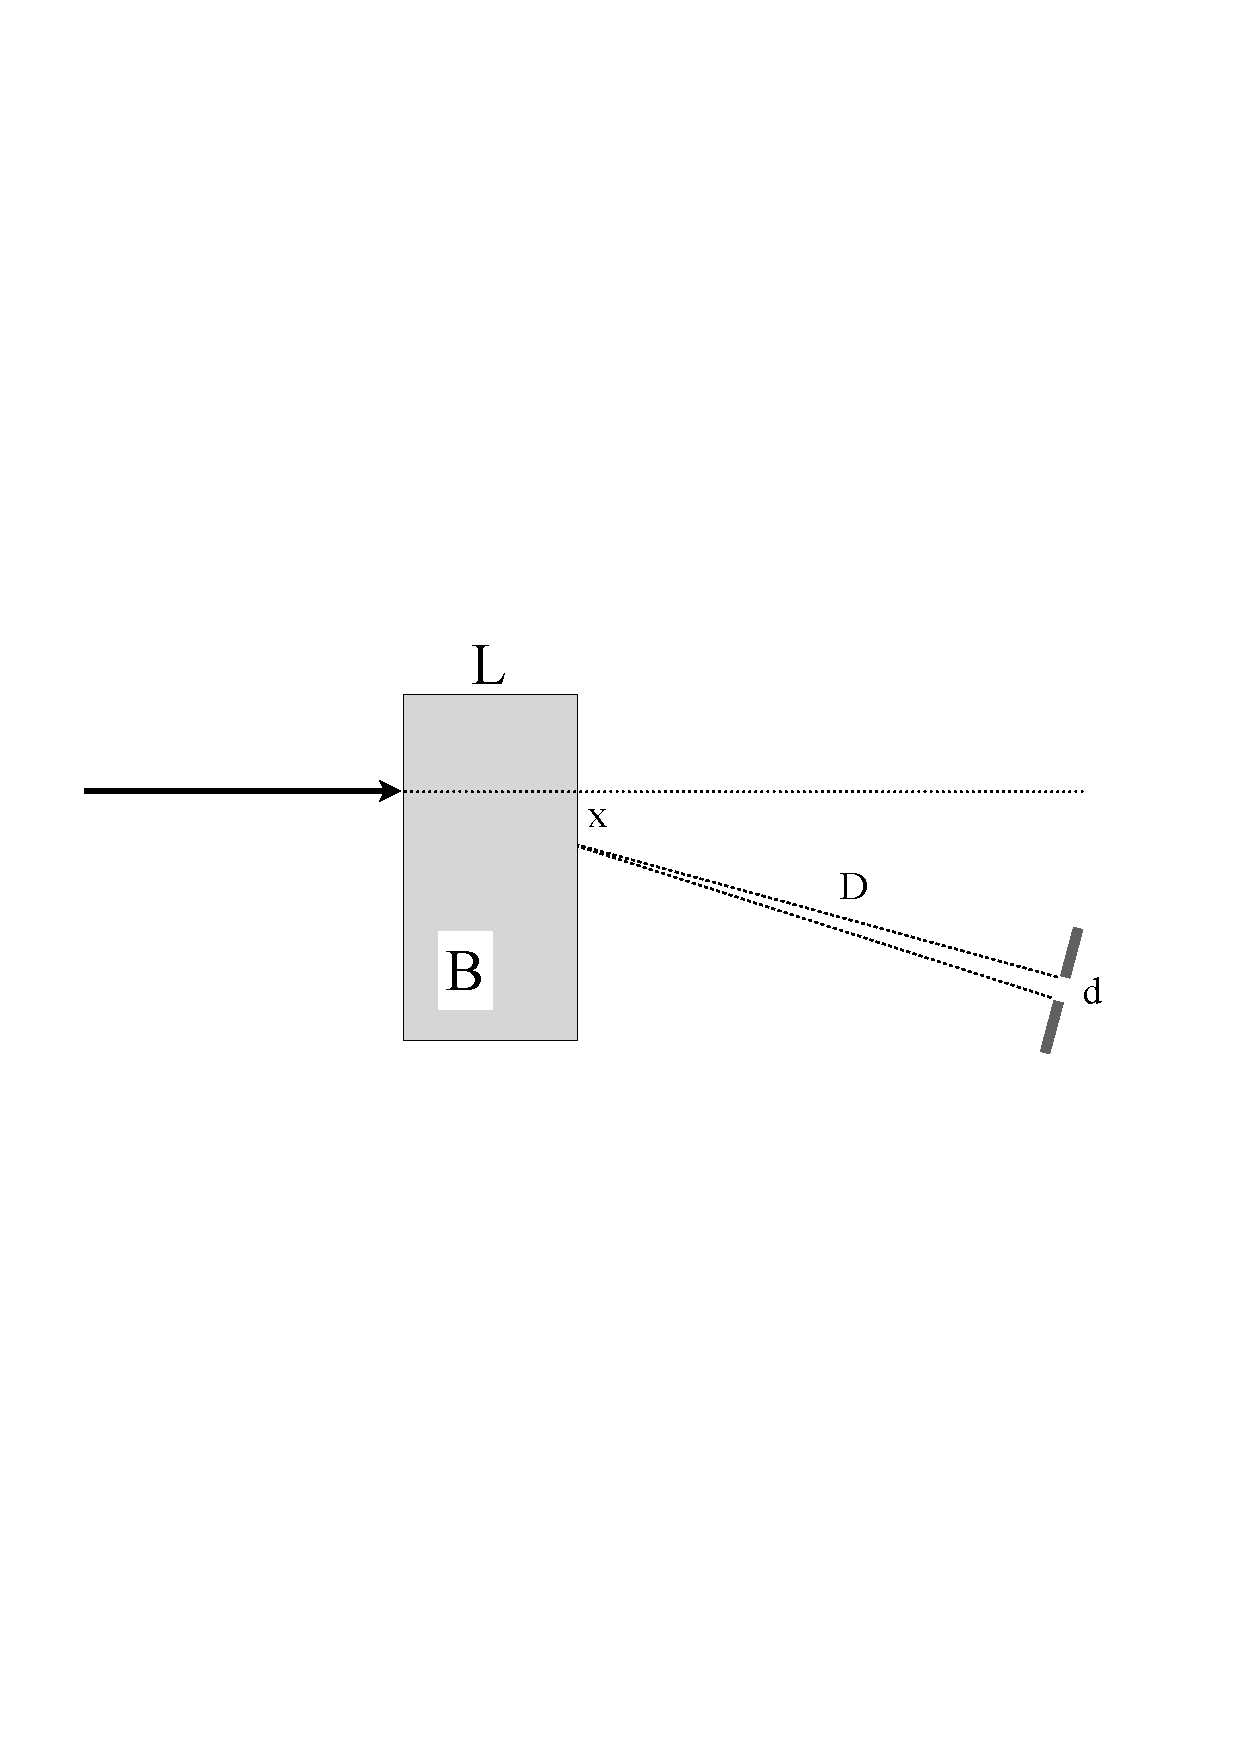
\includegraphics[width=0.49\linewidth]{fig-2021-04-07-fig1}
  \end{center}
  \end{figure}

  \Question A che distanza $x$ dalla linea di volo iniziale escono le particelle che hanno un impulso di \SI{2}{GeV/c}?   

  \Question Quale deve essere la larghezza minima $d$ del collimatore per selezionare particelle prodotte con momento entro $\pm 0.5\%$ dal valore centrale? Si trascuri la dipendenza di $x$ dall’impulso delle particelle.

  Posizionando dei contatori Cherenkov a soglia dopo il collimatore si vogliono identificare le particelle K+.

  \Question Quanti contatori Cherenkov sono necessari? Che valore di indice di rifrazione $n_i$ si pu\`o scegliere per ciascuno di essi (si consideri per tutte le particelle impulso pari a \SI{2}{GeV/c}).

  Si usino: $m_e = \SI{0.511}{MeV/c^2}$; $m_\mu = \SI{105}{MeV/c^2}$; $m_{\pi^+} = \SI{140}{MeV/c^2}$; $m_K = \SI{494}{MeV/c^2}$; $m_p = \SI{939}{MeV/c^2}$
\end{Exercise}
\begin{Answer}
  \begin{enumerate}
  \item In uno spettrometro magnetico vale:
    \[
    p[GeV] = 0.3B[T] R[m]
    \]
    pertanto le particelle con impulso $p = \SI{2}{GeV/c}$ si muovono su una circonferenza con raggio di curvatura:
    \[
    R = \frac{p}{0.3 \cdot B} = \SI{3.92}{m}.
    \]
    L’angolo di deflessione vale quindi:
    \[
    \theta = \arcsin (L/R),
    \]
    che per piccoli angoli si pu\`o approssimare ($\sin x \approx x per x \to 0$) con $\theta \approx L/R$. La distanza dalla linea di volo iniziale a cui escono le particelle \`e quindi:
    \[
    x = R(1-\cos\theta) \approx \frac{R\theta^2}{2} = \frac{L^2}{2R} = \SI{3.19}{cm}.
    \]
    
  \item L’impulso delle particelle selezionate dal collimatore sar\`a compreso tra:
    \begin{itemize}
    \item $p_1 = p\cdot(1-0.005) = \SI{1.99}{GeV/c}$ e
    \item $p_2 = p\cdot(1+0.005) = \SI{2.01}{GeV/c}$.
    \end{itemize}
    L’angolo formato da $p_1$ e $p_2$ all’uscita dal magnete vale:
    \[
    \Delta \theta = \theta_1 - \theta_2 = 0.3 \cdot B\cdot L\cdot (p_2 - p_1)/(p_1p_2) = \SI{1.27}{mrad}.
    \]
    Se la distanza della fenditura dall’uscita dal magnete \`e $D$, la sua larghezza minima deve essere
    \[
    d = D \cdot \Delta\theta = \SI{10}{m}\cdot\SI{1.27e-3}{rad} = \SI{1.27}{cm}.
    \]

  \item Affinch\'e venga emessa radiazione Cerenkov la velocit\`a di una particella deve essere tale che $\beta > 1/n$, quindi $n > 1/\beta$. I valori di $\beta$ per le particelle considerate e i corrispondenti indici di rifrazione minimi per avere emissione di radiazione sono:
    \begin{itemize}
      \item $e^+$: $\beta = 1$, quindi $n >1$
      \item $\mu^+$: $\beta = 0.9986$, quindi $n >1.0014$
      \item $\pi^+$: $\beta = 0.9976$, quindi $n >1.0025$
      \item $K^+$:, $\beta = 0.971$, quindi $n >1.030$
      \item protone: $\beta = 0.905$, quindi $n >1.105$
    \end{itemize}
    Per identificare i $K^+$ sono sufficienti due contatori Cherenkov con indici di rifrazione tali che nel primo siano sopra soglia $e^+$, $\mu^+$ e $\pi^+$, e nel secondo $e^+$, $\mu^+$, $\pi^+$ e
    $K^+$. Occorre quindi:
    \begin{itemize}
    \item un primo contatore con indice di rifrazione: $1.0025 < n <1.03$
    \item un secondo contatore con indice di rifrazione: $1.03 < n <1.105$
    \end{itemize}
    \`E preferibile scegliere valori dell’indice di rifrazione intermedi tra quelli indicati e non al limite. Valori ottimali sono ad esempio:
    \begin{align*}
      n_1 &= \left(\frac{\beta_{K^+} + \beta_\pi^+}{2}\right)^-1 = 1.016 \\
      n_2 &= \left(\frac{\beta_{K^+} + \beta_p}{2}\right)^-1 = 1.066
    \end{align*}
    L’anticoincidenza dei due segnali consente l’identificazione dei $K^+$.
  \end{enumerate}
\end{Answer}
